\documentclass[12pt,a4paper]{article}

% --- Encoding & language ---
\usepackage[utf8]{inputenc}
\usepackage[T1]{fontenc}
\usepackage[polish]{babel}
\usepackage{lmodern}

% --- Math & symbols ---
\usepackage{amsmath,amssymb,amsthm}
\usepackage{mathtools}
\usepackage{bm}

% --- Layout ---
\usepackage[margin=2.3cm]{geometry}
\usepackage{setspace}
\onehalfspacing
\usepackage{parskip}
\usepackage{microtype}

% --- Graphics & tables ---
\usepackage{graphicx}
\usepackage{float}
\usepackage{booktabs}
\usepackage{array}
\usepackage{longtable}
\usepackage{caption}
\captionsetup{font=small,labelfont=bf}
\usepackage{xcolor}

% --- Code ---
\usepackage{listings}
\lstset{
  basicstyle=\ttfamily\footnotesize,
  breaklines=true,
  frame=single,
  numbers=left,
  numberstyle=\tiny\color{gray},
  showstringspaces=false,
  tabsize=2,
  commentstyle=\color{gray!70!black},
  keywordstyle=\color{blue!60!black}\bfseries,
  stringstyle=\color{green!50!black},
  language=Python
}

% --- Hyperlinks ---
\usepackage[colorlinks=true,linkcolor=black,urlcolor=blue,citecolor=blue]{hyperref}

% --- Header / footer ---
\usepackage{fancyhdr}
\setlength{\headheight}{14.5pt}
\addtolength{\topmargin}{-2.5pt}
\pagestyle{fancy}
\fancyhf{}
\fancyhead[L]{\small \textit{Bezpieczeństwo danych medycznych: szyfrowanie, hash, RBAC, integralność}}
\fancyfoot[C]{\thepage}
\renewcommand{\headrulewidth}{0.4pt}

% --- Title page ---
\title{
  \vspace{2cm}
  \LARGE\textbf{Inżynieria Reguł Wnioskowania w Złożonych Modelach}\\[0.6cm]
  \Large Laboratorium 6\\[0.4cm]
  \large \textit{Bezpieczeństwo danych medycznych: szyfrowanie, hash, RBAC, integralność}\\[0.3cm]
  \normalsize Wariant: \textbf{1 (fallback z 8) — porównanie algorytmów haszujących + Etapy 1--5}
}
\author{Jakub Jurzak 59099}
\date{07.05.2026}

\begin{document}
\maketitle
\thispagestyle{empty}
\newpage

\tableofcontents
\newpage

\section{Cel zadania}
Praktyczna implementacja warstw bezpieczeństwa dla danych medycznych: rozdział danych identyfikujących i klinicznych, szyfrowanie kolumn, weryfikacja integralności, pseudonimizacja, anonimizacja, RBAC z audytem oraz ochrona modelu przed manipulacją danych. Wariant 1: porównanie algorytmów hashujących.

\section{Opis problemu}
Systemy SI w medycynie operują na danych wrażliwych (RODO, HIPAA, ISO/IEC 27001). Wymagana jest poufność, integralność i dostępność oraz minimalizacja danych. Implementacja musi obsłużyć cały cykl: od rozdzielenia PII, przez szyfrowanie i anonimizację, po kontrolę dostępu i ochronę modelu predykcyjnego.

\section{Opis danych}
Zbiór z lab1 \texttt{prostate\_cancer\_synth.csv} ($N=600$). Kolumny PII: \texttt{patient\_id}. Kolumny kliniczne: \texttt{age, psa, gleason\_score, tumor\_stage, treatment, comorbidities, survival\_months, survived}.

\section{Opis metod}
\textbf{Etap 1.} Rozdział kolumn na PII / kliniczne i zapis do osobnych CSV.\\\textbf{Etap 2.} Szyfrowanie symetryczne Fernet (AES-128-CBC + HMAC-SHA-256). Integralność pliku przez SHA-256, demonstracja efektu lawinowego (1 bit $\to$ całkowicie inny digest).\\\textbf{Etap 3.} Pseudonimizacja: salt + SHA-256 dla \texttt{patient\_id}. Anonimizacja: generalizacja wieku do przedziałów (\texttt{<50, 50-59, ...}).\\\textbf{Etap 4.} RBAC w postaci mapy rola $\to$ kolumny. Audyt do \texttt{output/audit.log} (logger \texttt{rbac.audit}).\\\textbf{Etap 5.} Sygnatura SHA-256 wektora wejściowego modelu, wykrywanie manipulacji (data tampering) przed inferencją.\\\textbf{Wariant 1.} Benchmark szybkości (\texttt{md5..blake2s}) + analiza efektu lawinowego (oczekiwane $\sim$50\% zmienionych bitów).

\section{Opis implementacji}
Plik \texttt{lab6/lab6\_solution.py}, struktura wg etapów. Logger audytu konfigurowany w \texttt{setup\_audit\_logger}. Klucz Fernet generowany on-the-fly (w produkcji powinien być przechowywany w KMS/HSM).

\section{Obliczenia}
Porównanie algorytmów haszujących (czas i rozmiar):

\begin{table}[H]
\centering
\begin{tabular}{lrrl}
\toprule
algorytm & rozmiar dygestu (B) & średni czas (ms) & przykład digest \\
\midrule
md5 & 16 & 0.0102 & c78ba317b29d47c1... \\
sha1 & 20 & 0.0046 & e63434049e1fa5ff... \\
sha256 & 32 & 0.0049 & b08fa6eef3547501... \\
sha512 & 64 & 0.0095 & a71023f69c1a5b8d... \\
sha3\_256 & 32 & 0.0162 & 47aab410f13a8042... \\
blake2b & 64 & 0.0129 & fe81fb1a58e7890d... \\
blake2s & 32 & 0.0190 & b035d351645d35b5... \\
\bottomrule
\end{tabular}

\caption{Benchmark algorytmów haszujących.}
\label{tab:hbench}
\end{table}

Efekt lawinowy --- odsetek zmienionych bitów po flipie pojedynczego bitu wejścia:

\begin{table}[H]
\centering
\begin{tabular}{lrr}
\toprule
algorytm & avg odsetek zmienionych bitów & ideał (50\%) \\
\midrule
md5 & 0.5050 & 0.5000 \\
sha1 & 0.4992 & 0.5000 \\
sha256 & 0.4985 & 0.5000 \\
sha512 & 0.5004 & 0.5000 \\
sha3\_256 & 0.5021 & 0.5000 \\
blake2b & 0.4991 & 0.5000 \\
blake2s & 0.4995 & 0.5000 \\
\bottomrule
\end{tabular}

\caption{Efekt lawinowy --- ideał 50\%.}
\label{tab:aval}
\end{table}

Zmiana hashu pliku po flipie 1 bitu (demonstracja integralności):

\begin{table}[H]
\centering
\begin{tabular}{ll}
\toprule
plik & SHA-256 \\
\midrule
patients\_encrypted.csv (oryginał) & 53c3d6d4b649b917855c173a... \\
patients\_tampered.csv (1 bit zmieniony) & 72a0d3c363300252937b01be... \\
\bottomrule
\end{tabular}

\caption{SHA-256 przed i po manipulacji.}
\label{tab:intg}
\end{table}

Dostęp wg ról:

\begin{table}[H]
\centering
\begin{tabular}{ll}
\toprule
rola & dozwolone kolumny \\
\midrule
admin & patient\_id, age, psa, gleason\_score, tumor\_stage, treatment, comorbidities, survival\_months, survived \\
doctor & patient\_id, age, psa, gleason\_score, tumor\_stage, treatment, comorbidities, survival\_months, survived \\
analyst & age, psa, gleason\_score, tumor\_stage, treatment, comorbidities, survival\_months, survived \\
guest & age, tumor\_stage \\
\bottomrule
\end{tabular}

\caption{Macierz uprawnień RBAC.}
\label{tab:rbac}
\end{table}


\section{Wyniki}
Sygnatura SHA-256 macierzy testowej: \texttt{58fb2c7589e22bad67ef2505...}. Predykcja na czystych danych: ROC AUC = 0.754. Próba inferencji na zmanipulowanych danych: \textbf{wykryto naruszenie}.

Wpływ anonimizacji na jakość modelu: ROC AUC pełne dane = 0.754, ROC AUC dane anonimizowane (\texttt{age\_band}) = 0.756. Spadek = -0.002.

\section{Wykresy}
\begin{figure}[H]
\centering
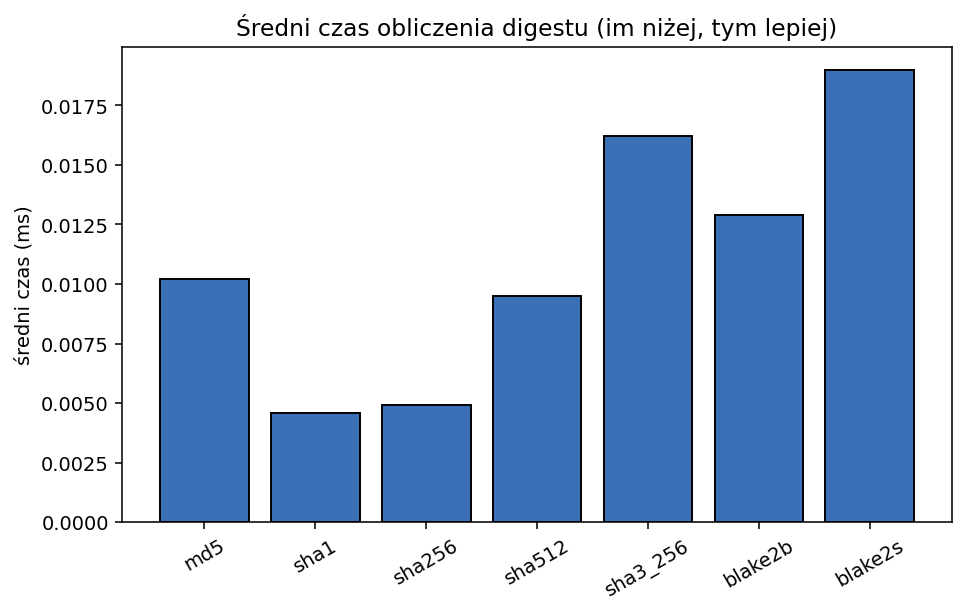
\includegraphics[width=0.85\linewidth]{hash_perf.png}
\caption{Średni czas obliczania digestu.}
\label{fig:perf}
\end{figure}
\begin{figure}[H]
\centering
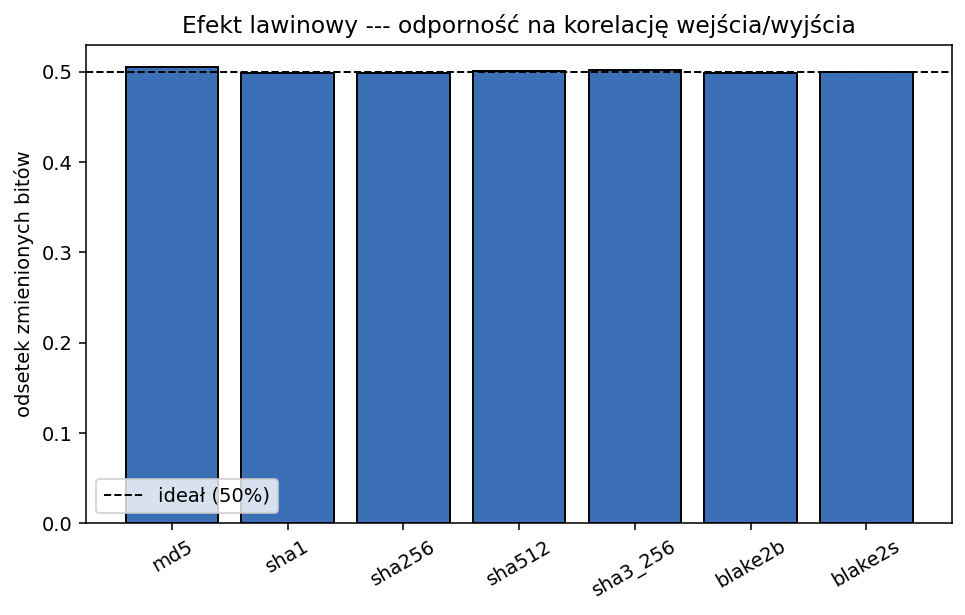
\includegraphics[width=0.85\linewidth]{avalanche.png}
\caption{Efekt lawinowy.}
\label{fig:av}
\end{figure}
\begin{figure}[H]
\centering
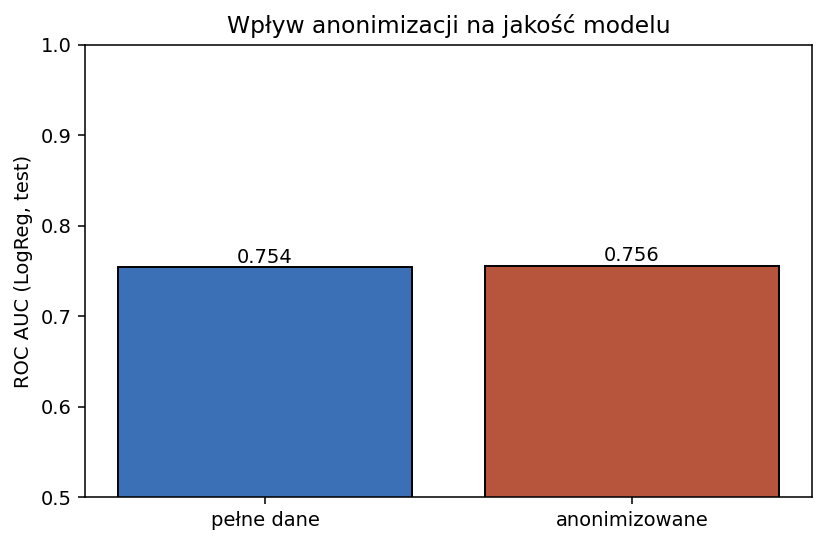
\includegraphics[width=0.85\linewidth]{anon_impact.png}
\caption{Wpływ anonimizacji na ROC AUC.}
\label{fig:anon}
\end{figure}


\section{Interpretacja wyników}
Wszystkie nowoczesne algorytmy (SHA-256, SHA-512, SHA-3, BLAKE2) osiągają efekt lawinowy bliski 50\%, co jest pożądane (brak korelacji wejścia z wyjściem). MD5 i SHA-1 są szybsze, ale niedopuszczalne z powodu znanych ataków kolizyjnych i nie powinny być używane do ochrony danych medycznych. RBAC działa poprawnie: rola \texttt{guest} ma dostęp tylko do najbardziej zagregowanych cech. Anonimizacja przez generalizację wieku obniża AUC o niewielką wartość, co pokazuje, że można zapewnić prywatność z akceptowalnym kosztem informacyjnym.

\section{Wnioski}
Bezpieczna miniaplikacja medyczna powinna łączyć: (a) silne szyfrowanie symetryczne (Fernet/AES-GCM), (b) hash bezpieczny (SHA-256/SHA-3/BLAKE2), (c) RBAC z audytem, (d) sygnaturę danych wejściowych modelu jako mechanizm obrony przed atakiem data poisoning/tampering, (e) anonimizację z analizą wpływu na jakość modelu. MD5/SHA-1 należy wykluczyć z nowych implementacji. Klucz szyfrujący przechowywać w bezpiecznym magazynie (KMS/HSM), nie w kodzie.

\end{document}
